 
\documentclass[12pt]{article}
 
\usepackage[margin=1in]{geometry} 
\usepackage{amsmath,amsthm,amssymb}
\usepackage{listings}

\usepackage[utf8]{inputenc}
\usepackage[norsk]{babel}

\usepackage{graphicx}
\usepackage{cleveref}

%\usepackage[parfill]{parskip}

\newenvironment{solution}{\begin{proof}[Løsning]}{\end{proof}}
 
\begin{document}
 
\title{Algoritmekonstruksjon: Øving 2}
\author{Simen Keiland Fondevik}

\maketitle

\section{Oppgave 1}
\it{\textbf{Skriv ut eksplisitt den grafiske matroiden for grafen i \Cref{matroid}.}}
\begin{figure}[ht]
  \begin{center}
  	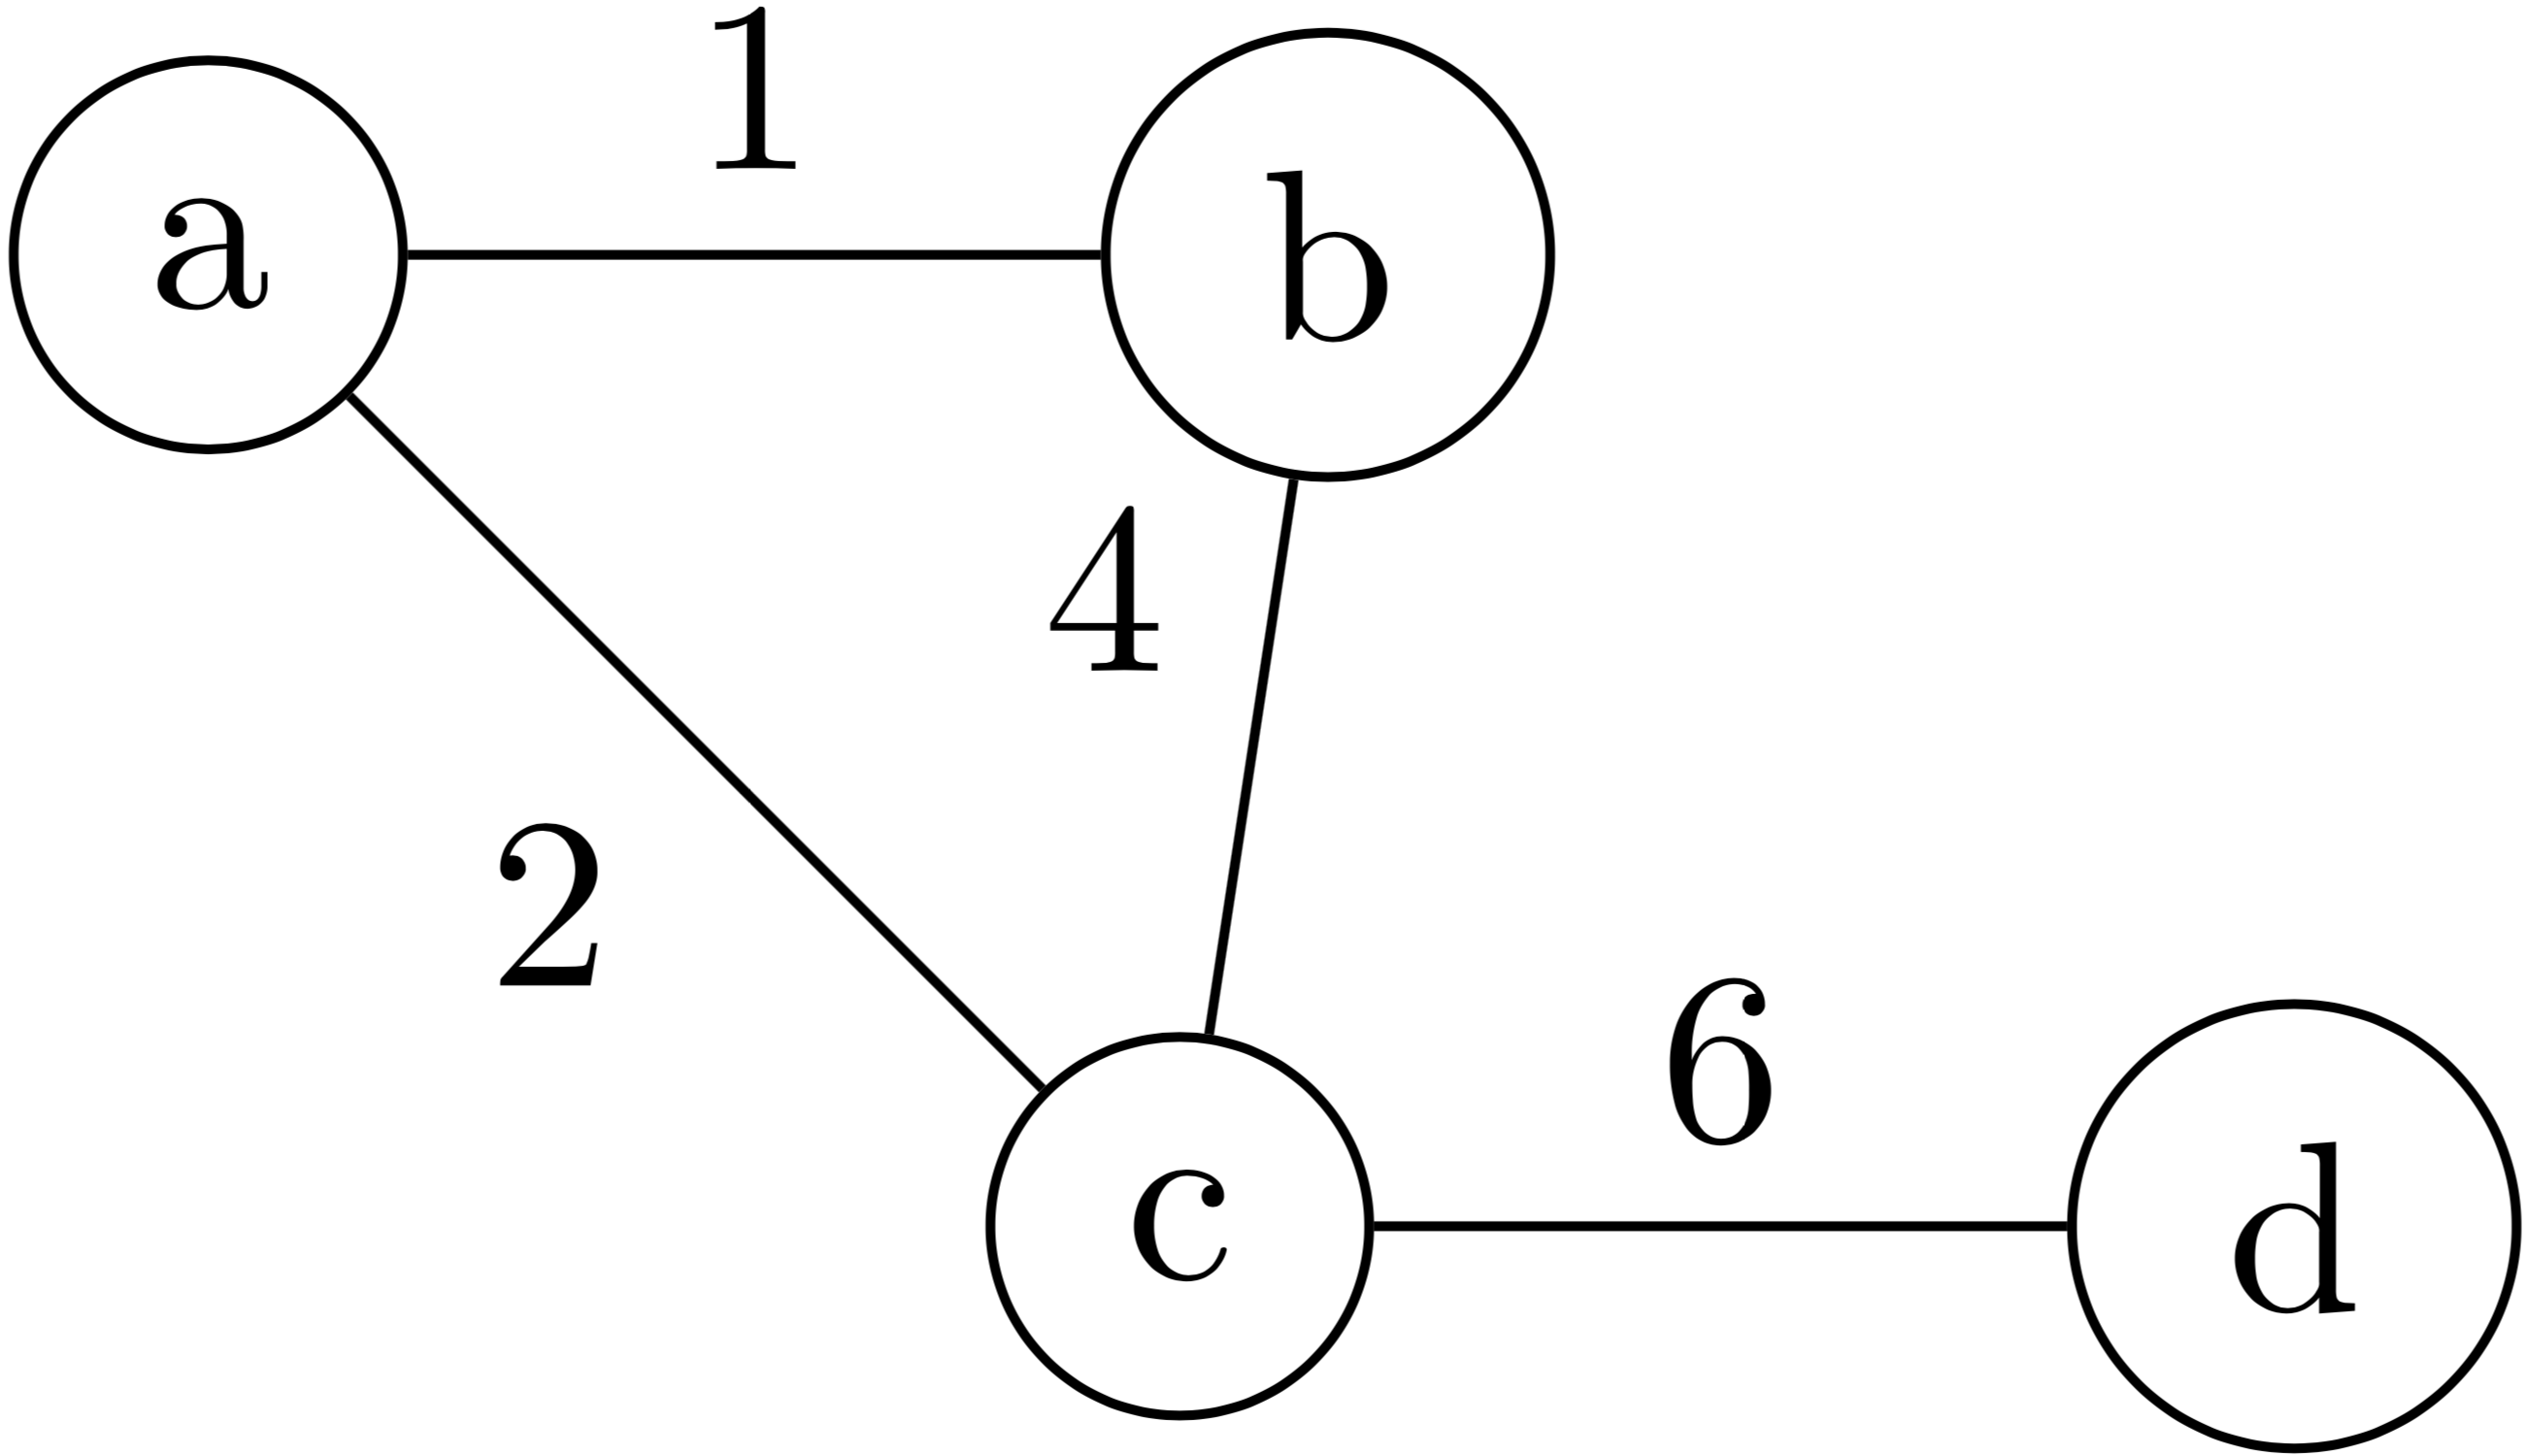
\includegraphics[width = 0.4\textwidth]{matroid.png}
    \caption{Graf for oppgave 1.}
    \label{matroid}
  \end{center}
\end{figure}

\begin{solution}
Den grafiske matroiden kan skrives som $M = (E, S)$ der $E$ er mengden av kanter i grafen og $S$ er alle delmengder av kanter som danner en skog i grafen. Det vil si,
\begin{align*}
E =& \{(a, b), ~(a, c), ~(b, c), ~(c, d)\} \\
S =& \{\{(a, b)\}, ~\{(a, c)\}, ~\{(b, c)\}, ~\{(c, d)\}, \\
   & \{(a, b), ~(b, c)\}, ~\{(a, b), ~(a, c)\}, ~\{(a, b), ~(c, d)\}, ~\{(b, c), ~(c, d)\} \\
   & \{(a, b), ~(a, c), ~(c, d)\}, ~\{(a, b), ~(b, c), ~(c, d) \}, ~\{(a, c), ~(b, c), ~(c, d)\} \}.
\end{align*}
\end{solution}

\it{\textbf{Skriv ut hva T er for hver iterasjon i den gråadige algoritmen anvendt på denne matroiden.}}
\begin{solution}
Den grådige algoritmen, gjengitt under, sorterer kantene i grafen etter ikke-økende vekter og velger grådig så fremt kanten ikke danner en sykel.
\begin{lstlisting}
GREEDY(E, S, w; T):
1.	order the elements of E according to their weight such that
	E = {e1, e2, ...em} with w(e1) >= w(e2) >= ... >= w(em);
2.	T = empty set;
3.	for k = 1 to m:
4.		if T + {ek} in S then T = T + {ek};
\end{lstlisting}
For vår instans velges altså kantene $(c, d)$, $(b, c)$ og $(a, c)$, i den rekkefølgen, dvs $T_0 = \emptyset$, $T_1 = \{(c, d)\}$, $T_2 = \{(c, d), ~(b, c)\}$, $T_3 = \{(c, d), ~(b, c), ~(a, c)\}$.
\end{solution}

\section{Oppgave 2}
\it{\textbf{Vis at matchingen i en graf $G$ generelt ikke danner en matroide, selv ikke når $G$ er bipartit.}}

\begin{proof}
Vi kan definere en matroide som et uavhengighetssystem der det tilhørende optimeringsproblemet løses korrekt med den grådige algoritmen over. Påstanden kan enkelt vises ved et moteksempel. La $G$ være den bipartitte grafen vist i \Cref{moteksempel}. Den grådige algoritmen vil velge kanten med vekt 3 og terminere. Dette er imidlertid ikke optimalt, da å velge de to andre kantene gir en samlet vekt på 4. Den grådige algoritmen feiler, og matching selv i bipartitte grafer
\begin{figure}[ht]
  \begin{center}
  	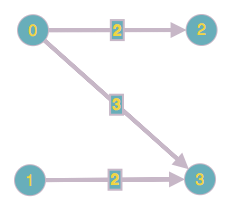
\includegraphics[width = 0.4\textwidth]{bipartite.png}
    \caption{Moteksempel for oppgave 2.}
    \label{moteksempel}
  \end{center}
\end{figure}
\end{proof}

\section{Oppgave 3}
\it{\textbf{La $G = (E, V)$ være en sammenhengende graf som ikke er et tre. Vis at delmengder av $E$ som inneholder ikke mer enn én sykel danner en matroide på $E$. Holder tilsvarende påstand om vi tillater to sykler?}}

\begin{proof}
Teorem 5.2.1 i Jungickel gir en ekvivalens mellom at $M$ er en matoride og at det for en hver $J, K \in S$ der $|J| = |K|+1$ alltid finnes et element $a \in J \backslash K$ slik at $K \cup \{a\} \in S$. Anta problemet danner en matroide. Det betyr at for en $J$ og $K$ i $S$ finnes et element $a$ som beskrevet over. Eneste måten $a$ ikke kan eksistere er hvis $K$ er en en delmengde av $J$ samtidig som det ekstra elementet i $J$ danner en ny sykel i $K$ om den legges til der (for ellers kunne en bare valgt som $a$ et hvilket som helst annet element i $J \backslash K$). Dette betyr imidlerid at J i utgangspunktet har to sykler, og dermed er $J \not\in S$. Vi har en selvmotisgelse, og dermed må problemet danne en matroide. (En kan eventuelt se på antall sammenkoplede komponenter i $J$ og $K$, der vi feks.vet at antall komponenter i K er $|V|-|K|+1$ hvis den har en sykel, og deretter bruke skuffeprinsippet og se at det alltid finnes en trygg kant å legge til).

Vi ser enkelt at samme argumentasjon kan generaliseres til at $S$ inneholder alle delmengder med et vilkårlig antall sykler.
\end{proof}


\section{Oppgave 4}
\it{\textbf{Vis at følgende algoritme er en $1/2$-approksimasjon for Knapsack.}}
Sorter først alle objektene etter synkende pris per størrelse slik at $v_1/s_1 \geq v_2/s_2 \geq \cdots \geq v_n/s_n$. La objektet med størst verdi betegnes $v^* = v_{i^*}$. Algoritmen velger de $k$ første objektene som får plass i sekken, slik at $\sum_{i=1}^{k}v_i \leq B$ og $\sum_{i=1}^{k+1} v_i \geq B$, der $B$ er kapasiteten til sekken. Returner $\max \left(i^{*}, ~ \{1, 2, \cdots k\} \right)$
\begin{proof}
Hvis vi kunne tatt med $k+1$ objekter ville vi fått verdien $\sum_{i=1}^{k+1} v_i > OPT$ der $OPT$ er den optimale løsningen på instansen. Ulikheten kommer av at algoritmen i grunn fungerer som den grådige, korrekte, algoritmen for fractional knapsack, der fractional knapsack som kjent alltid har en minst like høy målfunksjonsverdi som tilsvarende 0-1-innstans. Siden fractional knapsack bare ville fått plass til deler av element $k+1$, ville dens optimale verdi blitt $\sum_{i=1}^{k} v_i + \alpha \cdot v_{k+1} \geq OPT$ for en konstant $0 \leq \alpha < 1$. Venstresiden av denne likningen består av to ledd, slik at skuffeprinsippet gir at minst ett av dem er større enn eller lik $OPT/2$. Første ledd er normaltilfellet av algoritmen over, mens for det andre leddet har vi alltid $v_{k+1} \leq v^*$. Vi ser dermed at algoritmen alltid resturer noe som ikke er mindre enn halvparten av den optimale løsningen.
\end{proof}

\section{Oppgave 5}
\it{\textbf{Gitt følgende oppgaver å prosessere på formatet $(r_i, p_i)$ der $r_i$ er når oppgave $i$ blir tilgjengelig og $p_i$ er hvor lang tid det tar å utføre denne oppgaven. Hvilken oppgaveplan vil avrundingsalgoritmen generere, og hva er målverdien til denne løsningen?}} Instans: $(0, 10), ~(8, 1), (11, 2), ~(12, 2), ~(11, 3)$.

\begin{solution}
Avrundingsalgoritmen finner først en optimal løsning gitt at prosesser kan avbrytes og fortsettes på et senere tidspunkt. Dette kan gjøres i polynomtid med SRPT-regelen: Fra $t=0$ til $t=8$ gjøres deler av den første jobben. Deretter starter jobb 2, som fullføres ved $t=9$. Jobb 1 får så fortsette til den er ferdig ved $t=11$. Herfra starter jobb 3 siden denne vil fullføre først. Den er ferdig ved $t=13$. Til slutt gjøres jobb 4 og 5, i den rekkefølgen, og disse fullfører ved henholdsvis $t=15$ og $t=18$. Dette er altså optimalt hvis prosessene kan deles opp. Avrundingsalgorimen planlegger nå jobbene i stigende rekkefølge etter utregnede fullførelsestider over. Det vil si; fra $t=8$ til $t=9$ utføres jobb 2, fra $t=9$ til $t=19$ gjøres jobb 1, i intervallet (19, 21) utføres jobb 3, deretter jobb 4 fra $t=21$ til $t=23$ og til sist jobb 5 fra $t=23$ til $t=26$. Summen av sluttidene, som er målfunksjonen, blir da $9+19+21+23+26=98$.
\end{solution}

\it{\textbf{Hva er den optimale oppgaveplanen for instansen over, og hva er målverdien til denne løsningen?}}

\begin{solution}
Optimal planlegging vil for denne instansen være å utføre oppgavene i rekkefølgen de er oppgitt. Det git en verdi på målfunksjonen lik $10+11+13+15+18=67$.
\end{solution}

\it{\textbf{Lag en instans med minst tre oppgaver som overlapper der avrundingsal- goritmen vil gi optimalt svar.}}

\begin{solution}
En instans der vi kun har tre oppgaver som alle starter likt vil åpenbart løses optimalt med avrundingsalgoritmen.
\end{solution}


\section{Oppgave 6}
\it{\textbf{Avrundingsalgoritmen for mengdedekkeproblemet runder opp løsningene hvis $x_J^*\geq 1/f$. Vis at vi også får en $f$-approksimasjon ved å runde opp løsningene hvis $x_J^* > 0$.}}

\begin{proof}
Ved komplimentær slakkhet har vi at
\begin{equation*}
x_j^* > 0 \Rightarrow \sum_{i:e_i \in S_j} y_i^* = w_j.
\end{equation*}
Å ta med alle mengder der restriksjonen er stram, er det samme som gjøres i kapittel 1.4 \textit{Roudning a dual solution} i Williamson og Shmoys. Teorem 1.8 gir at algoritmen over er en $f$-approksimasjon.
\end{proof}

\end{document}
